
\section{Preservation of the Discrete Maximum Principle}

An important property for a discretization of the TRT equations is preservation of the
discrete maximum principle (MP).  The maximum principle states that the material temperature and mean intensity in the
interior of the domain should be bounded by the solution at the boundaries of the domain, in the
absense of interior energy sources~\cite{wollaber2013discrete,larsen_mpv}.  The analytic solution to the TRT equations satisfies a maximum
principle~\cite{larsen_mpv}, so we desire numerical approximations that preserve the MP in
a discrete sense, for each time step.
%For the discrete MP, we expect the numerical solution to be bounded by the boundary
%conditions at each time step.
For IMC simulations, violation of the maximum principle results in the material
temperature being artificially higher than the boundary conditions and sources should
physically allow.    As discussed in Sec.~\ref{sec:intro}, IMC can violate the MP due to
the approximate linearization of the emission source in the time discretization; it is not
truly implicit in time.  We expect our method, with a fully implicit time discretization,
to preserve the MP with sufficient convergence of the nonlinear emission
source~\cite{larsen_mpv}.

To numerically demonstrate that our method preserves the MP, we have simulated problems
similar to those in~\cite{wollaber2013discrete}.  We modify the Marshak wave problem in
Sec.~\ref{sec:marshak???}, by decreasing $c_v$ and increasing $\sigma_a$, to produce a
problem which results in MP violations for IMC at various fixed time step sizes. 
The spatial and temporal discretization determine the occurence of MP violations for
IMC. In particular, if time steps are too large or spatial
mesh cells are too small, IMC will demonstrate MP violations~\cite{wollaber2013discrete}.  Here, we have kept the
spatial mesh size fixed and increased time step to make MP violations occur.
The material
specifications for the problem are given in Table~\ref{tab:mpv_prob}. The domain width is 2.0 cm with
$N_c=150$ uniform spatial mesh cells.  The radiation and material energies are initially in
equilibrium at $0.01$ keV, before an isotropic boundary source of $1$ keV is applied at
the left boundary at $t=0$. The simulation is ran unitl $t=0.1$ sh. 

The material and radiation temperature are plotted for an IMC simulation with $\Delta
t=0.025$ sh in
Figure~\ref{fig:imc_mpvrad}.  Figure~\ref{fig:imc_mpv} depicts the material temperature
for various time step sizes and a fixed mesh size of 150 equally spaced cells.     All IMC
simulations used 100,000 histories per time step. As demonstrated in
Fig.~\ref{fig:imc_mpvrad}, the material temperature exceeds the specified boundary
temperature and is artificially hotter than the radiation temperature.  This artificial
``temperature spike'' also leads to a slower propagation of the
wave~\cite{wollaber2013discrete}.  As shown in
Fig.~\ref{fig:imc_mpv}, as larger timestep sizes are taken the nonphysical results worsen.
It is noted that although the final solution for $\Delta t=0.0001$ sh obeys the MP, during
the first few time steps the temperature spikes are present.

The simulations are repeated with the same specifications for the HOLO method. All HOLO
simulations used a fixed mesh of 8 $\mu$ cells by 150 $x$ cells, 3 batches per time step,
and 6,000 histories per batch.  As seen in
Figure~\ref{fig:holo_mpv}, the TRT solution does not violate the maximum principle.
For these simulaitons, it was
necessary to use a damped Newton's method to converge the solutions.  A damping factor of
0.5 was used for all these simulations, and found to stably converge.

Table~\ref{tab:mpv_iters} demonstrates the LO Newton iteration counts for the HOLO method.
For reference, the solution at $\Delta t = 0.00001$ sh requires no damping.  Clearly
damping increases the number of iteration counts per step as the Newton solve is taking
more conservative steps, but the overall increase is not dramatic. 





NO FIXUP APPLIED, NEWTON CONVERGENCE OF 10e-06.  MODIFIED MARSHAK WAVE PROBLEM.


\begin{figure}[H]
    \centering
    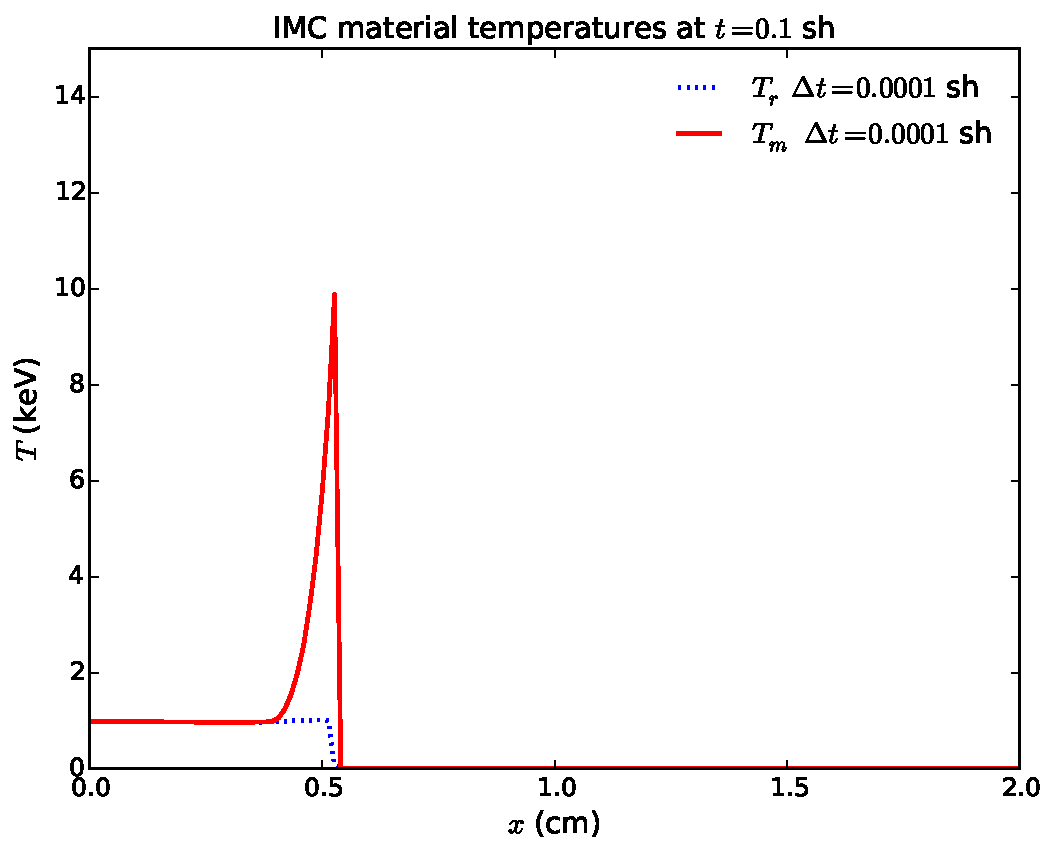
\includegraphics[width=0.6\linewidth]{mpv_rad_imc.pdf}
    \caption{\label{fig:imc_mpvrad}Simulation of MP violation problem with IMC method and $\Delta t = 0.001$ sh.}
\end{figure}

\begin{figure}[H]
    \centering
    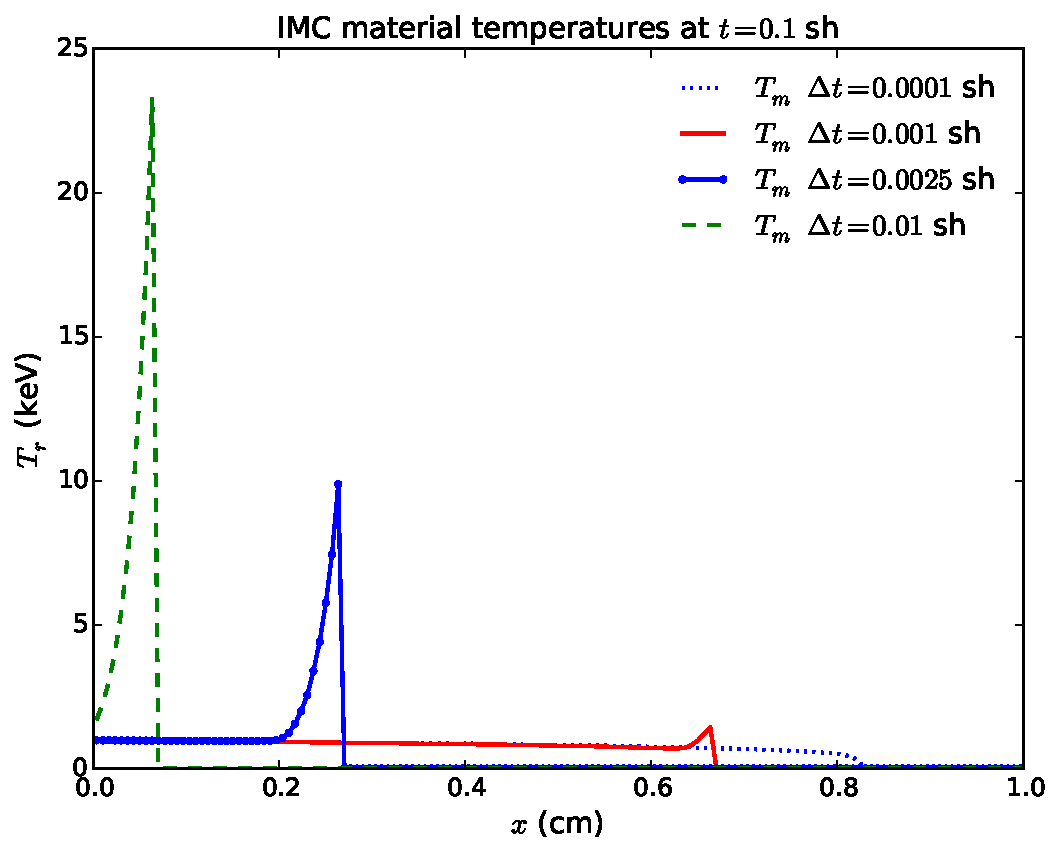
\includegraphics[width=0.6\linewidth]{mpv_mats_imc.pdf}
    \caption{\label{fig:imc_mpv}Simulation of MP violation problem with IMC method for various time step
    sizes.}
\end{figure}

\begin{figure}[H]
    \centering
    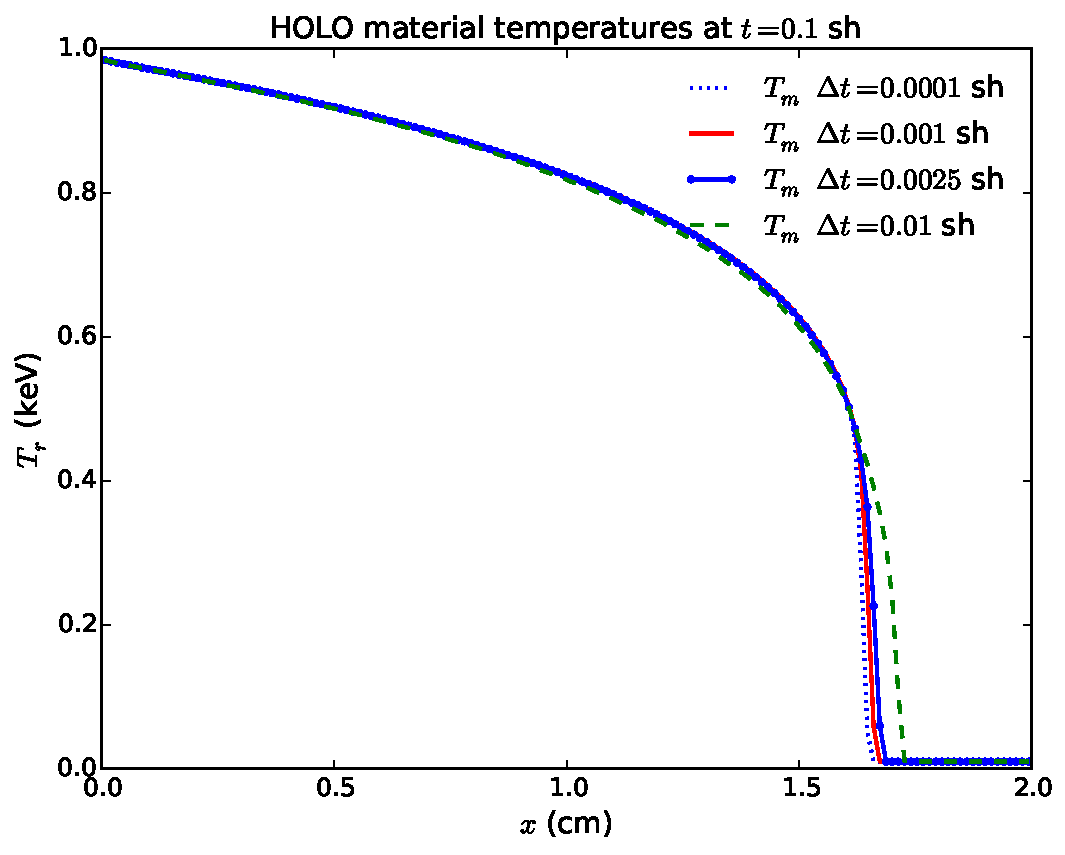
\includegraphics[width=0.6\linewidth]{mpv_mats_holo.pdf}
    \caption{\label{fig:holo_mpv}Simulation of MP violation problem with HOLO-ECMC method for various time step
    sizes.}
\end{figure}



\begin{table}[H]
        \caption{\label{tab:mpv_prob}Problem specifications for maximum principle
        violation. Absorption cross section has form $\sigma_a = \sigma_{a,0}/T^3$.}
\centering
        \begin{tabular}{|c|c|} \hline
            $\sigma_{a,0}$ (cm$^{-1}$ keV$^3$)  & 4.0  \\ 
            $\sigma_s$ (cm$^{-1}$) & 0.0 \\
            $\rho$ (g cm$^{-3}$) & 1.0  \\
            $c_v$ (jks/keV-g) & 0.0081181  \\ \hline
        \end{tabular}
\end{table}

\begin{table}[H]
    \caption{\label{tab:mpv_iters}Comparison of LO Newton iterations for different time
step sizes and MP problem. For $\Delta t=0.1$, damping has $\zeta = 1$.  For all other
cases $\zeta = 0.5$.}  
    \centering
        \begin{tabular}{|cc|} \hline
            $\Delta t$ & Avg. Iters / Time Step \\
            $\sigma_s$ (cm$^{-1}$) & 0.0 \\
            $\rho$ (g cm$^{-3}$) & 1.0  \\
            $c_v$ (jks/keV-g) & 0.0081181  \\ \hline
        \end{tabular}
\end{table}



   An isotropic incident intensity of 0.150 keV is applied
at $x=0$; the incident intensity on the right boundary is $2.5\times10^{-5}$ keV.
The material properties are $\rho = 1$ g cm$^{-3}$ and $c_v = 0.013784$ jks/keV-g. The
absorption cross section varies as $\sigma(T) = 0.001\;\rho\; T^{-3}$ (cm$^{-1}$).
The simulation was advanced until $t=5$~sh~(1~sh~$\equiv$~10$^{-8}$~s) with a fixed time step size of 0.001 sh. For comparison purposes, we
have not used adaptive mesh
refinement, only performed one HOLO iteration per time
step, and use a fixed 3 HO batches with equal number of histories per batch. A
relative tolerance of $10^{-6}$ for the change in $\phi(x)$ and $T(x)$ was used for
the LO newton solver for all results. Radiation energy
distributions are plotted as an equivalent temperature given by
$T_r=(\phi/(ac))^{0.25}$.  Cell-averaged quantities are plotted.
Although isotropic scattering can be included in the LO solver with this method~\cite{ans_2014}, we have only
considered problems with $\sigma_s = 0$ here.  
